% Derived from the template file for the LaTeX package SVJour3
% for Springer journals.          Springer Heidelberg 2010/09/16
%
% This template includes a few options for different layouts and
% content for various journals. Please consult a previous issue of
% your journal as needed.
%
% First comes an example EPS file -- just ignore it and
% proceed on the \documentclass line
% your LaTeX will extract the file if required
\begin{filecontents*}{example.eps}
%!PS-Adobe-3.0 EPSF-3.0
%%BoundingBox: 19 19 221 221
%%CreationDate: Mon Sep 29 1997
%%Creator: programmed by hand (JK)
%%EndComments
gsave
newpath
  20 20 moveto
  20 220 lineto
  220 220 lineto
  220 20 lineto
closepath
2 setlinewidth
gsave
  .4 setgray fill
grestore
stroke
grestore
\end{filecontents*}

%INCLUDE SPEEDUP CSV HERE

\RequirePackage{fix-cm}
%
%\documentclass{svjour3}                     % onecolumn (standard format)
\documentclass[smallcondensed]{svjour3}     % onecolumn (ditto)
%\documentclass[smallextended]{svjour3}       % onecolumn (second format)
%\documentclass[twocolumn]{svjour3}          % twocolumn
%
\smartqed  % flush right qed marks, e.g. at end of proof
%
\usepackage{graphicx}
%
% \usepackage{mathptmx}      % use Times fonts if available on your TeX system
%
% insert here the call for the packages your document requires
\usepackage{csvsimple}
\usepackage[inline, shortlabels]{enumitem}
\usepackage{epstopdf}
\usepackage{hyperref}
\usepackage{mathtools}
\usepackage{tikz}
\usetikzlibrary{arrows, calc, decorations.pathreplacing, positioning,
  shapes.geometric}
% etc.

% please place your own definitions here and don't use \def but
% \newcommand{}{}

\newcommand{\etal}{{\em et al.}}

% For example theory of lists
\newcommand{\Zero}{\text{Z}}
\newcommand{\Succ}{\text{S}}

\newcommand{\List}{\text{List}}
\newcommand{\ListA}{\text{List} \  a}
\newcommand{\Nil}{\text{Nil}}
\newcommand{\Cons}{\text{Cons}}
\newcommand{\Head}{\text{head}}
\newcommand{\Tail}{\text{tail}}
\newcommand{\Append}{\text{append}}
\newcommand{\Reverse}{\text{reverse}}
\newcommand{\Length}{\text{length}}
\newcommand{\Map}{\text{map}}
\newcommand{\Foldl}{\text{foldl}}
\newcommand{\Foldr}{\text{foldr}}

% Insert the name of "your journal" with
\journalname{Journal of Automated Reasoning}

\begin{document}

\title{Quantitative Benchmarking for Automatically Generated Conjectures%\thanks
% {Grants or other notes about the article that should go on the front page
% should be placed here. General acknowledgments should be placed at the end of
% the article.}
}
% \subtitle{Do you have a subtitle?\\ If so, write it here}

% \titlerunning{Short form of title}        % if too long for running head

\author{Chris Warburton \and
        Alison Pease    \and
        Jianguo Zhang}

% \authorrunning{Short form of author list} % if too long for running head

\institute{C. Warburton \at
           University of Dundee \\
           \email{c.m.warburton@dundee.ac.uk} \\
           ORCID: 0000-0002-4878-6319 \\
           Phone: +44 (0)1382 386968
%             \emph{Present address:} of F. Author  %  if needed
           \and
           A. Pease \at
           University of Dundee \\
           \email{a.pease@dundee.ac.uk} \\
           ORCID: 0000-0003-1856-9599
           \and
           J. Zhang \at
           University of Dundee \\
           \email{j.n.zhang@dundee.ac.uk} \\
           ORCID: 0000-0001-9317-0268
}

\date{Received: date / Accepted: date}
% The correct dates will be entered by the editor

\maketitle

\begin{abstract}
  We propose a benchmarking methodology to evaluate the efficiency and quality
  of \emph{conjecture generation} by automated tools for \emph{mathematical
    theory exploration}. Our approach uses widely available theorem proving
  tasks as a \emph{ground-truth} corpus, and we demonstrate its use on the
  QuickSpec and IsaCoSy tools. We found that both may fail, even for small
  inputs, but QuickSpec usually finishes in significantly less time than IsaCoSy
  and produces significantly more ``interesting'' output. By defining a standard
  benchmark we provide a measure of progress for the field, encourage
  innovation through healthy competition and allow direct comparisons to be made
  between the disparate approaches currently being pursued for this task.
  \keywords{Theory Formation \and Theorem Proving \and Lemma Discovery \and Conjecture Generation \and Benchmarking}
% \PACS{PACS code1 \and PACS code2 \and more}
% \subclass{MSC code1 \and MSC code2 \and more}
\end{abstract}

\begin{acknowledgements}
  We are grateful to the authors of the systems we have used in our experiments,
  especially for help in obtaining and configuring their tools. We would
  especially like to thank Koen Claessen, Lucas Dixon, Moa Johansson, Dan
  Ros\'{e}n and Nicholas Smallbone for useful discussions and help in adapting
  their software to our purposes.

  This work was supported by the Engineering and Physical Sciences Research
  Council grant EP/P017320/1 and studentship 1526504.
\end{acknowledgements}

\pagebreak

\section{Introduction}
\label{intro}

\emph{Conjecture generation} is the open-ended task of conjecturing properties
of a given logical theory which are somehow ``interesting'', and is
studied as a sub-field of \emph{mathematical theory exploration} (MTE). This has
applications wherever we find uses for formal methods: in proof assistants and
their libraries, in mathematics education and research, and in the specification
and verification of software. Although formal methods, and automated reasoning
more generally, have been advocated in mathematics (notably by
Voevodsky~\cite{voevodsky2010univalent} and Gowers~\cite{ganesalingam2013fully})
and software engineering (for example via dependently-typed
programming~\cite{McKinna:2006}), they have a reputation for being difficult and
expensive, which has historically limited their use to high-assurance domains
such as aerospace and microprocessor design.

One path to reducing these barriers is to increase the level of automation.
Software verification tools have been shown to benefit from the addition of a
conjecture generation step for finding ``background lemmas'', which are useful
when proving user-provided statements~\cite{Claessen.Johansson.Rosen.ea:2013}.
Another path is to tailor the division of labour between humans and machines
such that each is playing to their strengths, which has been referred to as
``centaur teams''~\cite{harari2017reboot,davenport2015beyond}. Machines can
systematically search a much larger space of possible relationships than humans,
potentially bringing to light novel and surprising connections, whilst allowing
the user to make the ultimate judgement over which of the most promising results
are worth investigating further.

Similar tasks are also studied in the domain of Computational \emph{Scientific}
Discovery~\cite{king2004functional,Williams20141289,schmidt2009distilling}, for
example in the search for new drugs. The major difference between scientific and
mathematical discovery is that inductive reasoning and experimental testing are,
in principle, more important for the former, although we note that they are also
core principles in the mathematical tools we have investigated (in particular
for ensuring the \emph{plausibility} of conjectures).

We limit ourselves to mathematical applications, but even here it is difficult
to measure and compare the success of approaches and tools. This is partially
due to their diversity, but also because of the inherent ambiguity of the task
(what counts as ``interesting''?), the different goals emphasised by their
designers and the variety of evaluation methods employed. We attempt to solve
this discrepancy, at least for the foreseeable future, by defining a standard,
unambiguous benchmarking approach with which to compare the conjecture
generation of MTE tools. Our contributions include:

\begin{itemize}
\item A general methodology for benchmarking conjecture generation.
\item Resolving the issue of ``interestingness'' through the use of
  theorem-proving benchmarks as a ground-truth.
\item A specific instantiation of this methodology, using the Tons of Inductive
  Problems (TIP) benchmark as a corpus.
\item Automated tooling to perform this benchmarking.
\item Application of our methodology to the QuickSpec and IsaCoSy MTE tools,
  and a comparison and discussion of the results.
\end{itemize}

We describe the conjecture generation problem in more detail, along with the
difficulty of comparing existing solutions, in $\S$\ref{sec:background}. We
explain our proposal for a more general benchmark in $\S$\ref{sec:proposal} and
demonstrate its application to existing MTE tools in $\S$\ref{sec:application}.
Issues facing our approach, and the field in general, are discussed in
$\S$\ref{sec:discussion}; related work is surveyed in
$\S$\ref{sec:related-work}, including the diverse terminology found in the
literature; and concluding remarks are given in $\S$\ref{sec:conclusion}.

\begin{sloppypar}
  Our benchmark implementation is available at
  \url{http://chriswarbo.net/projects/theory-exploration} and
  \url{https://github.com/warbo}. All processes, including benchmark generation,
  experimental runs and generation of this paper, are specified using the
  Nix~\cite{dolstra2004nix} system to aid reproducibility.
\end{sloppypar}

\section{Background}
\label{sec:background}

\subsection{Motivation}
\label{sec:motivation}

\begin{figure}
  \begin{equation*}
    \begin{split}
      \forall a. \Nil            &: \ListA                                  \\
      \forall a. \Cons           &: a \rightarrow \ListA \rightarrow \ListA \\
      \Head(\Cons(x, xs))        &= x                                       \\
      \Tail(\Cons(x, xs))        &= xs                                      \\
      \Append(\Nil,         ys)  &= ys                                      \\
      \Append(\Cons(x, xs), ys)  &= \Cons(x, \Append(xs, ys))               \\
      \Reverse(\Nil)             &= \Nil                                    \\
      \Reverse(\Cons(x, xs))     &= \Append(\Reverse(xs), \Cons(x, \Nil))   \\
      \Length(\Nil)              &= \Zero                                   \\
      \Length(\Cons(x, xs))      &= \Succ (\Length(xs))                     \\
      \Map(f, \Nil)              &= \Nil                                    \\
      \Map(f, \Cons(x, xs))      &= \Cons(f(x), \Map(f, xs))                \\
      \Foldl(f, x, \Nil)         &= x                                       \\
      \Foldl(f, x, \Cons(y, ys)) &= \Foldl(f, f(x, y), ys)                  \\
      \Foldr(f, \Nil,         y) &= y                                       \\
      \Foldr(f, \Cons(x, xs), y) &= f(x, \Foldr(f, xs, y))
    \end{split}
  \end{equation*}
  \caption{A simple theory defining a $\List$ type and some associated
    operations, taken from~\cite{Johansson.Dixon.Bundy:conjecture-generation}.
    $\Zero$ and $\Succ$ are from a Peano encoding of the natural numbers}
  \label{figure:list_theory}
\end{figure}

Given a logical theory, such as the theory of lists shown in
Figure~\ref{figure:list_theory}, we may want to find properties (e.g.
invariants) describing its behaviour. This could be for mathematical curiosity,
or due to the theory's importance in some domain. In particular, when dealing
with definitions in a software library, we may regard a set of such properties
as the code's \emph{specification}. Even those properties which only hold by
coincidence, rather than by design, may still be useful for \emph{optimising}
uses of this library, by rewriting expressions into equivalent forms which
require less time, memory, network usage, etc. For example, our theory of lists
turns out to satisfy the following invariant:

\begin{equation} \label{eq:mapreduce}
  \forall f. \forall xs. \forall ys.
    \Map(f, \Append(xs, ys)) = \Append(\Map(f, xs), \Map(f, ys))
\end{equation}

Whilst these two expressions produce equivalent results, the form on the right
can execute both calls to $\Map$ in parallel (in a pure functional language, at
least); a fact which is exploited by the ``map/reduce'' parallel programming
paradigm.

Such use cases require the ability to \emph{discover} true properties of some
particular definitions; this requires not only \emph{proving} their correctness,
but also \emph{posing} them as conjectures in the first place. This is a hard
problem in general, but presents opportunities for automation due to the
precise, symbolic nature of the domain. These processes can also feed into each
other, since proven properties can be used as lemmas for subsequent proofs. As
an example, proving Equation~\ref{eq:mapreduce} may require ``background
knowledge'', such as the property $\forall x. \Append(x, \Nil) = x$, which may
be tedious to produce by hand but possible to discover automatically.

\subsection{Automating Construction and Exploration of Theories}
\label{sec:te}

The task of automatically proving or disproving a \emph{given} conjecture has
been studied extensively in the field of Automated Theorem Proving (ATP). Less
attention has been paid to \emph{generating} such conjectures automatically,
either from a given set of definitions (the task we will focus on) or where the
definitions are also generated. This research has been pursued under the names
of Automated Theory Formation (ATF) and Mathematical Theory Exploration (MTE);
we will use the MTE terminology, and discuss their relationship further in
$\S$\ref{sec:related-work}.

A major challenge when generating conjectures is choosing how to narrow down the
resulting set to only those deemed ``interesting'', since this is an imprecise
term with many different interpretations. For example, all existing approaches
agree that simple tautologies are ``uninteresting'', but differ when it comes to
more complex statements.  Colton \etal{} surveyed tools for theory formation
and exploration, and their associated notions of ``interestingness'' for
concepts and conjectures~\cite{colton2000notion}. Six qualities were identified,
which are applied to conjectured properties as follows:

{\bf Empirical plausibility} checks whether a property holds across some
specific examples. This is especially useful for avoiding falsehoods, without
resorting to a deductive proof search.

{\bf Novelty} depends on whether the property, or one isomorphic or more
general, has already been seen.

{\bf Surprisingness} of a property is whether or not it is ``obvious'', for
example if it is an instance of a tautology.

{\bf Applicability} depends on the number of models in which a
property holds. High applicability makes a property more interesting, but so
does zero applicability (i.e. non-existence).

{\bf Comprehensibility} depends on the syntactic complexity of the property's
statement. Simpler statements are considered more interesting (which favours
tools adopting a small-to-large search order).

{\bf Utility} is the relevance or usefulness of a property to the user's
particular task. For example, if we want to find properties which are useful for
optimisation, like Equation~\ref{eq:mapreduce}, then utility would include
whether the property justifies some rewrite rule, the difference in resource
usage of the expressions involved, and how common those expressions are in real
usage.

Attempting to \emph{measure} such qualities is difficult, and having too many
measures complicates comparisons. System developers have employed a more
practical alternative in their evaluations, which is to perform
\emph{precision/recall} analysis against a \emph{ground-truth}. This requires
choosing a set of definitions (such as those in Figure~\ref{figure:list_theory})
and a set of properties (the ground truth) which represent the ``ideal'' result
of conjecture generation for those definitions (e.g. this might include
Equation~\ref{eq:mapreduce}). To analyse the quality of a tool's conjectures, we
run it on these chosen definitions and compare its output to the ground truth:

\begin{itemize}
\item \emph{Precision} is the proportion of a tool's output which appears in
  the ground truth (the ratio of true positives to all positives). This
  penalises overly-liberal tools which output a large number of properties in
  the hope that some turn out to be ``good''.
\item \emph{Recall} is the proportion of the ground truth which appears in the
  tool's output (the ratio of true positives to actual positives). This
  penalises overly-conservative tools which generate very few properties as a
  way to avoid ``bad'' ones.
\end{itemize}

To score 100\% on precision and recall, all of the properties which appear in
the ground truth must have been conjectured, and nothing else. This gives us a
simple method to evaluate and compare tools without requiring a general solution
to the question of what is ``interesting''; although we must still decide what
to put in the ground truth set, and what to leave out, for each measured set of
definitions.

\begin{sloppypar}
  The precision and recall of three MTE tools are compared
  in~\cite{claessen2013automating}:
  IsaCoSy~\cite{Johansson.Dixon.Bundy:conjecture-generation},
  IsaScheme~\cite{Montano-Rivas.McCasland.Dixon.ea:2012} and
  HipSpec~\cite{Claessen_hipspec:automating}.\footnote{Unfortunately this
    comparison only reports prior results for each tool, rather than reproducing
    them. This makes the numbers less comparable, since each tool was tested
    with slightly different definitions (e.g. whether or not the exponential and
    maximum functions were included).} The definitions and ground truths for all
  three were taken from the standard library of the Isabelle proof assistant.
  The fact that the library authors expended the effort of stating, proving and
  bundling these properties with every copy of their software is a good
  indication that they are interesting. Two sets of definitions were used: a
  theory of natural numbers; and a theory of lists (which we show in
  Figure~\ref{figure:list_theory} on page~\pageref{figure:list_theory}). With
  only two datapoints, each containing only a few definitions and properties (4
  functions and 12 properties, in the natural number example), it is difficult
  to draw general conclusions; yet despite these limitations we believe that
  this is a viable method to performing meaningful, objective analyses and
  comparisons for such tools. It is only with larger data sets that we can
  generalise the measured performance to different, especially \emph{novel},
  domains (which, after all, is the purpose of MTE tools). In addition, we might
  be concerned that such ``popular'' theories as the natural numbers may be
  unrepresentative of typical usage. For example, we would not expect the
  library functions in a typical verification problem to be as mathematically
  rich as number theory.
\end{sloppypar}

\subsection{Existing Tools}
\label{sec:existing-tools}

Since our benchmarking methodology builds on the precision/recall analysis
described in $\S$\ref{sec:te}, we decided to use two of the same tools, IsaCoSy
and QuickSpec (the conjecture generating component of HipSpec), as our
demonstration.

IsaCoSy (Isabelle Conjecture Synthesis) is written for the Isabelle proof
assistant, mostly in Standard
ML~\cite{Johansson.Dixon.Bundy:conjecture-generation}. It conjectures equations
by enumerating expressions involving a given set of (typed) constants and free
variables (a \emph{signature}). A constraint solver forbids certain
(sub)expressions from being synthesised, and these constraints are extended
whenever a new property is conjectured, to avoid generating any special-cases of
this property in the future. Conjectures are tested by looking for
counterexamples and, if none are found, sent to IsaPlanner which attempts to
prove them.

QuickSpec emerged from work on the QuickCheck software testing framework for the
Haskell programming language~\cite{claessen2011quickcheck}. As well as
conjecturing properties of Haskell definitions for HipSpec, it has been applied
to Isabelle definitions via the Hipster tool~\cite{Hipster}. Like IsaCoSy,
QuickSpec takes a signature and enumerates well-typed terms. It collects
together those of the same type into equivalence classes, assuming them to be
equal, then uses QuickCheck to find counterexamples to this assumption by
randomly instantiating the variables and comparing the resulting closed
expressions. Any equivalence class whose elements don't compare equal are split
up, and the process is repeated with new random values.

After 500 rounds of testing, any expressions still sharing the same equivalence
class are conjectured to be equal for all values of their variables. Rather than
using a constraint system to prevent redundancies (such as special-cases of
other properties), QuickSpec instead passes its output through a congruence
closure algorithm to achieve the same effect.

\section{Theory Exploration Benchmark}
\label{sec:proposal}

Our main contribution is a benchmarking methodology, shown in
Figure~\ref{figure:flow_chart} on page~\pageref{figure:flow_chart}, which both
generates a large definition/ground-truth corpus, and provides a scalable,
statistical approach to evaluating MTE tools using this corpus. We follow a
precision/recall approach similar to prior work, with the main difference being
the source of definitions and ground truths: we take existing problem sets
designed for automated theorem proving, and adapt their content for use in the
conjecture generation setting.

\subsection{Preparation}
\label{section:prep}

Automated theorem proving is an active area of research, with large problem sets
and regular competitions to prove as much as possible, as fast as
possible~\cite{pelletier2002development}. These problem sets are an opportunity
for MTE, as their definitions and theorems can be used as a corpus in the same
way that Isabelle libraries have been used in the past.

Some problem sets are more amenable for this purpose than others. The most
suitable are those meeting the following criteria:

\begin{itemize}
\item For each problem, there should be a clear distinction between the
  statement to be proved and the definitions involved, such that the two can be
  easily and meaningfully separated. This rules out problem sets like those of
  SMT-COMP~\cite{barrett2005smt}, where many problems involve uninterpreted
  functions, whose behaviour is \emph{implicit} in the logical structure of the
  theorem statement but not separately \emph{defined}.
\item Definitions should be translatable into a form suitable for the MTE tools
  under study. Our application in $\S$\ref{sec:application} requires Haskell and
  Isabelle translations, and also benefits from having definitions be strongly
  typed.
\item The problem set should be relevant to the desired domain. We focus on pure
  functional programming, which requires higher-order functions and inductively
  defined datatypes, which rules out first-order languages/logics (such as
  TPTP~\cite{sutcliffe2009tptp}).
\item The problem set should ideally contain \emph{every} ``interesting''
  property involving its included definitions, since non-membership in the
  ground truth will be treated as being ``uninteresting''. More realistically,
  we should aim for each definition to have \emph{multiple} properties; rather
  than a mixture of unrelated problems, cherry-picked from different domains.
\item Larger problem sets are preferable as they give more robust statistics, all
  else being equal (i.e. when this does not sacrifice quality).
\end{itemize}

Once such a problem set has been chosen, we must separate the definitions from
the theorem statements which reference those definitions. The definitions will
be used as input to the MTE tools, whilst the theorem statements form the ground
truth corpus of properties (which tool output will be compared against).

It is important to ensure that there are no duplicate definitions: we are only
concerned with the \emph{logical} content of the input, not the more arbitrary
aspects of their presentation like the names of functions. For example, consider
a problem set which includes a statement of commutativity for a \texttt{plus}
function, and of associativity for an \texttt{add} function, where the
definitions of \texttt{plus} and \texttt{add} are $\alpha$-equivalent. We would
expect an MTE tool to either conjecture commutativity and associativity for
\emph{both} functions, or for \emph{neither} function, since they are logically
equivalent. Yet a na\"ive precision/recall analysis would treat commutativity of
\texttt{add} and associativity of \texttt{plus} as \emph{uninteresting}, since
they don't appear in the ground truth.

For this reason, duplicates should be removed, and any references to them
updated to use the remaining definition (e.g. chosen based on lexicographic
order). In the above example, the \texttt{plus} function would be removed, and
the commutativity statement updated to reference \texttt{add} instead.

\subsection{Sampling}
\label{section:sampling}

We could, in theory, send these de-duplicated definitions straight into an MTE
tool and use the entire set of properties (taken from the theorem statements) as
the ground truth for analysis. However, this would cause two problems:

\begin{itemize}
\item The result would be a single data point, which makes it difficult to
  infer performance \emph{in general}.
\item It is impractical to run existing MTE tools on inputs containing more
  than a few dozen definitions.
\end{itemize}

To solve both of these problems we instead \emph{sample} a subset of
definitions.\footnote{This could be done randomly, but for reproducibility we
  use a deterministic order based on cryptographic hashes.} Given a sample size,
we choose a subset of that many definitions, and provide only those as input to
the tool. We generate a corresponding ground truth by selecting those properties
from the corpus which ``depend on'' (contain references to) \emph{only} the
definitions in that sample. Transitive dependencies aren't required (e.g. a
property involving only a \texttt{times} function would not depend on a
\texttt{plus} function, even if \texttt{plus} occurs in the definition of
\texttt{times}).

Unfortunately, uniform sampling of definitions gives rise to a lottery: for a
given sample size, increasing the size of the corpus (which provides better
statistics) makes it less likely that a chosen sample will contain all of
a property's dependencies. The majority of such samples would hence have an
empty ground truth, and thus $0$ precision and undefined recall
\emph{independent} of the tool's output! This is clearly undesirable as an
evaluation method.

Other measurements could be used for such cases, but our approach is to avoid
them by only allowing a sample if it contains all dependencies of at least one
property. We could do this using rejection sampling, but it is more efficient to
pick a property, weighted in proportion to their number of dependencies
(ignoring those with more dependencies than our sample size). That property's
dependencies become our sample, padded up to the required size with uniform
choices from the remaining definitions.

The ground truth for such samples is guaranteed to contain at least one property
(the one we picked), and hence the precision and recall will depend meaningfully
on the tool's output. One downside of this restriction is that we limit the
number of possible samples to measure; this is significant for sample sizes less
than~3.

\subsection{Evaluation}
\label{section:evaluation}

Given a sample of definitions and a corresponding ground truth, the actual
execution of the MTE tool proceeds as in prior work. We must translate the
chosen definitions into the required input format, then we time the execution
with a timeout (e.g. 5 minutes). We use wall-clock time since
\begin {enumerate*} [i) ]%
\item this is most relevant to a user's experience,
\item it has a straightforward interpretation and
\item measuring it does not require intrusive alterations to a tool's
  implementation.
\end {enumerate*}
The downside is that comparisons must take hardware performance into account,
which would not be the case if time were measured by some proxy like number of
expressions evaluated.

In our experiments we have found that memory usage is also an important part of
a tool's performance, but rather than complicating our analysis with an extra
dimension, we instead allow programs to use as much memory as they like, and
either get killed by the operating system or slow down so much from swapping
that they time out. This is in line with the expected usage of these tools:
either there is enough memory, or there isn't; implementations should not be
penalised for making use of available resources.

To calculate precision and recall, the conjectures generated by each tool, as
well as the ground-truth properties, need to be parsed into a common format and
compared syntactically after normalising away ``irrelevant'' details. We
consider variable naming to be irrelevant, which can be normalised by numbering
free variables from left to right and using de Bruijn indices for bound
variables. We also consider the left/right order of equations to be irrelevant,
which we normalise by choosing whichever order results in the
lexicographically-smallest expression.

We specifically \emph{ignore} other logical relationships between syntactically
distinct statements, such as one equation being implied by another. Whilst
logically sound, second-guessing the ground truth in this way would harm other
aspects which influence interestingness (for example, a more general statement
is more widely applicable, but it might also be harder to comprehend).

This procedure gives us, for each sample, a set of generated conjectures and a
set of ground truth properties (from which precision and recall can be
calculated) and a single runtime. We propose two methods for analysing this
data: \emph{summarising} the performance of a single MTE tool and
\emph{comparing} the performance of two tools.

\subsection{Summarising}

Each sample is only explored once by each tool, so that we cover as many
independent samples as possible to better estimate how a tool's performance
generalises to unseen inputs. How we combine these data into an aggregate
summary depends on what we are interested in measuring. One general question we
might ask is how a tool's performance scales with respect to the input size (the
number of given definitions). This is straightforward to measure by varying the
sample size, but we need some way to combine the results from samples of the
same size.

We can summarise a set of runtimes by choosing the median, as this is more
robust than the mean against long-running outliers, and hence represents
performance for a ``typical'' input of that size. Since our methodology measures
performance over many samples, we can also compute the \emph{spread} of our
data, for example the inter-quartile range. This is not possible using the
one-off measurements common in prior evaluation methods.

Precision and recall are ratios, which can be averaged (separately) in two ways,
known as the \emph{Average of Ratios} (AoR) and the \emph{Ratio of Averages}
(RoA)~\cite{egghe2012averages}. The Average of Ratios is the mean value. Using
the definitions of precision and recall given in $\S$\ref{sec:te}, we can define
their means for $S$ samples indexed by $1 \leq i \leq S$ as follows:

\begin{align*}
       \overline{\text{precision}}_{AoR}
    &= \frac{1}{S} \sum_i{\text{precision}_i} \\
    &= \frac{1}{S} \sum_i{
         \frac{\#\text{interesting}_i}
              {\#\text{generated}_i}}         \\[10pt]
       \overline{\text{recall}}_{AoR}
    &= \frac{1}{S} \sum_i{\text{recall}_i} \\
    &= \frac{1}{S} \sum_i{
         \frac{\#\text{interesting}_i}
              {\#\text{groundtruth}_i}}
\end{align*}

We interpret these mean values as the \emph{expected} precision and recall for
samples of this size. In particular, these tell us the quality of the \emph{set}
of conjectures that will be generated if we were to run the tool on such a
sample, but they don't give us direct information about the individual
conjectures themselves. Since these are mean values, they are the reference
point for measures of spread such as the variance, standard deviation and mean
absolute deviation.

The Ratio of Averages is \emph{pooled}, combining the (multi)sets from each
sample before taking the ratios. The size of these pooled sets is simply the sum
of the individual set sizes, and ratios of these sums are equal to ratios of the
means (since the normalising factor $\frac{1}{S}$ appears in both numerator and
denominator):

\begin{align*}
       \overline{\text{precision}}_{RoA}
    &= \frac{\sum_i{\#\text{interesting}_i}}
            {\sum_i{\#\text{generated}_i}}                              \\
    &= \frac{\frac{1}{S} \sum_i{\#\text{interesting}_i}}
            {\frac{1}{S} \sum_i{\#\text{generated}_i}}                  \\
    &= \frac{\hspace{5pt} \overline{\#\text{interesting}} \hspace{5pt}}
            {\hspace{5pt} \overline{\#\text{generated}}   \hspace{5pt}} \\[10pt]
       \overline{\text{recall}}_{RoA}
    &= \frac{\sum_i{\#\text{interesting}_i}}
            {\sum_i{\#\text{groundtruth}_i}}                            \\
    &= \frac{\frac{1}{S} \sum_i{\#\text{interesting}_i}}
            {\frac{1}{S} \sum_i{\#\text{groundtruth}_i}}                \\
    &= \frac{\hspace{5pt} \overline{\#\text{interesting}} \hspace{5pt}}
            {\hspace{5pt} \overline{\#\text{groundtruth}} \hspace{5pt}}
\end{align*}

Larger sets contribute more to a Ratio of Averages, unlike the mean which treats
each set equally. This weighting gives us expected qualities of
\emph{conjectures} rather than sets: the RoA for precision is the expected
chance that some particular generated conjecture will appear in the ground
truth; the RoA for recall is the expected chance that some particular ground
truth property will appear in the generated output.

These averages can differ when there is a large variation in set size. For
example, if we generate a single, interesting conjecture for one sample and 99
uninteresting conjectures for another sample, the AoR (mean) precision will be
$\frac{1}{2}$ but the RoA precision will be $\frac{1}{100}$. This highlights the
importance of knowing \emph{absolute} numbers of conjectures, such as the mean
output size $\overline{\#\text{generated}}$ and its spread, alongside the
proportions given by precision and recall.

It is also possible to combine precision values \emph{with} recall values
(either individually or aggregated) by calculating their \emph{F-score}, defined
as:

\begin{equation*}
  F = 2 \times \frac{\text{precision} \times \text{recall}}
                    {\text{precision} +      \text{recall}}
\end{equation*}

This is the harmonic mean of precision and recall, ranging between 0 and 1. The
F-score summarises performance into a single number, which is useful for
purposes like ranking, but it obscures insights we might gain from looking at
precision and recall separately (e.g. whether a tool is generating too much
output or too little).

\subsection{Comparison}

To measure progress and encourage competition in the field, it is important to
compare the relative performance of different tools on the same task. Since the
aggregate statistics in the above summaries have obscured the details of
specific runs, any comparison based on them (such as comparing mean recall)
would have very low statistical power. More direct comparisons can be made using
\emph{paired} tests, since for each individual sample we have measurements for
\emph{both} tools.

Running times do not follow a normal distribution, in particular due to the
lower bound at 0, which complicates any application of standard comparisons like
the paired z-test. An alternative which does not assume normality is the
Wilcoxon signed-rank test~\cite{wilcoxon1945individual}, which has been applied
to software benchmarking in the Speedup-Test protocol of Touati, Worms and
Briais~\cite{touati2013speedup}. Our methodology differs by measuring with a
different sample each time, rather than repeatedly measuring one sample of each
size; measuring both tools on the \emph{same} samples allows the paired form of
the Wilcoxon test to be used.

Another complication with our time measurements is the censoring effect caused
by timeouts. Paired difference tests are robust to this, since the upper-bound
on total time imposes an upper-bound to the observable difference; this biases
our conclusions in a conservative way, \emph{towards} the null hypothesis of
indistinguishable performance.

Quality can be compared using precision and recall, but we must choose how to
handle samples where one tool succeeded and the other failed (e.g. by timing
out). Failed runs can be treated as if they had succeeded with an empty set of
conjectures; this penalises failure-prone tools and simplifies analysis by
ensuring every sample produces a data point. An alternative is to discard
samples which caused either tool to fail, and compare only those where both
tools finished successfully. We follow this second approach, since it is more
charitable to the tools being evaluated (which, after all, were not designed
with our benchmark in mind). With fewer data points to analyse, we pool together
samples of all sizes (allowing duplicates) and compare proportions from these
aggregations.

Recall relies on a fixed set of properties, the ground truth, so we can compare
tools using McNemar's test for paired samples~\cite{mcnemar1947note}. For each
tool, we count how many of the ground-truth properties it found which were
\emph{not} found by the other tool; i.e. those occasions where one tool was
objectively better than the other. McNemar's test determines whether we can
reject the null hypothesis that both counts are the same.

Comparing precision cannot be done in the same way as recall, since we do not
have a fixed set of properties to compare both tools on (there are an unlimited
number of properties that may or may not appear in each tool's output). Instead,
we can count how many of the generated conjectures were interesting and
uninteresting for each tool, and use Boschloo's form of Barnard's
test~\cite{lydersen2009recommended} to determine if these proportions are
independent. This assumes that precision follows a binomial distribution, and
the test is conditioned on the number of generated conjectures (as if this were
fixed by design, rather than determined by the tool).

\begin{figure}
  \centering
  \tikzstyle{startstop} = [rectangle, rounded corners, minimum width=3cm,
                           minimum height=1cm,text centered, draw=black]

  \tikzstyle{io} = [trapezium, trapezium left angle=70,
                    trapezium right angle=110, minimum width=1cm,
                    minimum height=1cm, text centered, draw=black]

  \tikzstyle{process} = [rectangle, minimum width=3cm, minimum height=1cm,
                         text centered, draw=black]
  \tikzstyle{decision} = [diamond, minimum width=3cm, minimum height=1cm,
                          text centered, draw=black]

  \tikzstyle{arrow} = [thick,->,>=stealth]

  % Avoids too much padding in io shapes
  \tikzset{trapezium stretches=true}

  \begin{tikzpicture}[node distance=1cm]

    % Preparation section

    \node (in)  [io]{Theorem Proving Benchmark};
    \node (sep) [process,       below=1cm of in         ]{Separate definitions from property statements};
    \node (def) [process, below  left=1.5cm and -1cm of sep]{Remove duplicate definitions};
    \node (ref) [process, below right=1.5cm and -1cm of sep]{Update references};

    \node (thy)  [startstop, below=1cm of def]{Distinct Definitions};
    \node (thm)  [startstop, below=1cm of ref]{Corpus of Properties};

    \draw [arrow] (in)  -- (sep);
    \draw [arrow] (def) -- (ref);
    \draw [arrow] (def) -- (thy);
    \draw [arrow] (ref) -- (thm);

    % Arrows with labels
    \path[->]
        (sep) edge [arrow, sloped, above] node {definitions} (def)
        (sep) edge [arrow, sloped, above] node {properties}  (ref);

    % Sampling section

    \node (choose) [process, below=of thm   ]{Choose a property};
    \node (deps)   [process, below=of choose]{List property's dependencies};

    % Create dummy coordinate below deps, then use its y coordinate for pad
    \coordinate [below=of deps] (padDummy);
    \path let \p{dummy} = (padDummy),
              \p{in}    = (in)
              in coordinate (padPos) at (\x{in}, \y{dummy});
    \node (pad)  [process, at=(padPos)]{Pad list to form sample};

    \node (sthm) [startstop, below right=1.5cm and -1cm of pad]{Ground Truth};
    \node (sthy) [startstop, below  left=1.5cm and -1cm of pad]{Sampled Theory};


    % Calculate position of (size) using let, then define as normal
    \path let \p{pad}    = (pad),
              \p{choose} = (choose)
           in coordinate (sizePos) at (\x{pad},\y{choose});
    \node (size) [io, at=(sizePos)] {Sample size};

    % Evaluation section
    \path let \p{pad}  = (pad),
              \p{sthm} = (sthm)
           in coordinate (runPos) at (\x{pad}, \y{sthm});
    \node (run) [process, below=of runPos]{Run MTE tool};
    \node (pr)  [process, below=of run]{Analysis};

    \node (prec) [startstop, below=of pr  ]{Precision};
    \node (time) [startstop,  left=of prec]{Time taken};
    \node (rec)  [startstop, right=of prec]{Recall};

    \draw [arrow] (thy)    |- (pad);
    \draw [arrow] (thm)    -- (choose);
    \draw [arrow] (choose) -- (deps);
    \draw [arrow] (deps)   |- (pad);
    \draw [arrow] (size)   -- (choose);
    \draw [arrow] (size)   -- (pad);
    \draw [arrow] (pad)    -- (sthm);
    \draw [arrow] (pad)    -- (sthy);
    \draw [arrow] (sthy)   |- (run);
    \draw [arrow] (run)    -- (pr);
    \draw [arrow] (sthm)   |- (pr);
    \draw [arrow] (pr)     -- (prec);
    \draw [arrow] (pr)     -- (rec);
    \draw [arrow] (pr)     -- (time);

    % Awkward arrow
    \draw [arrow] (thm) -| ([shift={(7mm,-7mm)}]thm.east) |- (sthm);

    % Braces

    % Preparation
    \draw
      let \p{thm} = (thm.east),
          \p{in}  = (in.north),
          \p{rec} = (rec.south east)
       in [decorate,decoration={brace, amplitude=10pt}, xshift=0.5cm]
       (\x{rec}, \y{in}) -- (\x{rec}, \y{thm})
         node [black, midway, right, xshift=0.3cm]
              {Preparation $\S$\ref{section:prep}};

    % Sampling
    \draw
      let \p{thm} = (thm.east),
          \p{gt}  = (sthm.east),
          \p{rec} = (rec.south east)
       in [decorate,decoration={brace, amplitude=10pt}, xshift=0.5cm]
       (\x{rec}, \y{thm}) -- (\x{rec}, \y{gt})
         node [black, midway, right, xshift=0.3cm]
              {Sampling $\S$\ref{section:sampling}};

    % Evaluation
    \draw
      let \p{sthm} = (sthm.east),
          \p{rec}  = (rec.south east)
       in [decorate,decoration={brace, amplitude=10pt}, xshift=0.5cm]
       (\x{rec}, \y{sthm}) -- (\x{rec}, \y{rec})
         node [black, midway, right, xshift=0.3cm]
              {Evaluation $\S$\ref{section:evaluation}};

  \end{tikzpicture}
  \caption[]{High-level view of the benchmarking methodology described in
    $\S$\ref{sec:proposal}, showing
    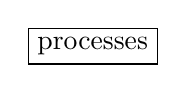
\begin{tikzpicture}
      \node [rectangle, text centered, draw=black]{processes};
    \end{tikzpicture},
    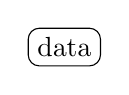
\begin{tikzpicture}
      \node [rectangle, rounded corners, text centered, draw=black]{data};
    \end{tikzpicture} and
    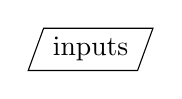
\begin{tikzpicture}
      \node [trapezium, trapezium left angle=70, trapezium right angle=110,
             text centered, draw=black]{inputs};
  \end{tikzpicture}}
  \label{figure:flow_chart}
\end{figure}

\section{Application}
\label{sec:application}

We have applied our benchmarking methodology to the QuickSpec and IsaCoSy MTE
tools, using version 0.2 of the TIP (Tons of Inductive Problems) theorem proving
benchmark as our ground truth corpus~\cite{claessen2015tip}.

To determine our benchmarking parameters we ran some initial tests on both tools
for a few samples sized between 1 and 100, for an hour each on our benchmarking
machine with a 3.2GHz dual-core Intel i5 processor with hyper-threading and 8GB
of RAM. Most QuickSpec runs either finished within 200 seconds or not at all,
and sizes above 20 mostly timed out. IsaCoSy mostly finished within 300 seconds
on sample sizes up to 4, but by size 8 was mostly timing out; its few successes
above this took thousands of seconds each, which we deemed infeasibly long.

Based on this we decided to benchmark sample sizes up to 20, since neither tool
seemed to perform well beyond that. The Speedup-Test protocol follows the
statistical ``rule of thumb'' of treating sample sizes $\leq$ 30 as ``small'',
so we pick 31 samples of each size in order to cross this threshold. This gave a
total of 1240 runs. To keep the benchmarking time down to a few days we chose a
timeout of 300 seconds, since that covered most of the successful QuickSpec and
IsaCoSy results we saw, and longer times gave rapidly diminishing
returns. During analysis, duplicate samples (caused by our requirement that
samples have a non-empty ground truth) were found and discarded, so only 14
samples of size 1 were used and 30 of size 2.

\subsection{Tons of Inductive Problems}
\label{sec:tip}

We chose the Tons of Inductive Problems (TIP) benchmark for our ground truth
since it satisfies the criteria specified in $\S$\ref{section:prep}: each
benchmark problem has standalone type and function definitions, making their
separation trivial; known examples from the software verification and inductive
theorem proving literature are included, ensuring relevance to those fields; the
format includes the higher-order functions and inductive datatypes we are
interested in; it is large enough to pose a challenge to current MTE tools; plus
it is accompanied by tooling to convert its custom format (an extension of
SMT-Lib~\cite{BarFT-SMTLIB}) into a variety of languages, including Haskell and
Isabelle.

We use TIP version 0.2 which contains 343 problems, each stating a single
property and together defining a total of 618 datatypes and 1498 functions. Most
of these are duplicates, since each problem (re\nobreakdash-)defines all of the
datatypes and functions it involves.

TIP datatypes can have several ``constructors'' (introduction forms) and
``destructors'' (elimination forms; field accessors). For example the type of
lists from Figure~\ref{figure:list_theory} can be defined in the TIP format as
follows:

\begin{samepage}
\begin{verbatim}
(declare-datatypes
  (a)                       ;; Type parameter (element type)
  ((List                    ;; Type name
     (Nil)                  ;; Constructor (nullary)
     (Cons                  ;; Constructor (binary)
       (head a)             ;; Field name and type
       (tail (List a))))))  ;; Field name and type
\end{verbatim}
\end{samepage}

Our target languages (Haskell and Isabelle) differ in the way they handle
constructors and destructors, which complicates comparisons. To avoid this, we
generate a new function for each constructor (via $\eta$-expansion) and
destructor (via pattern-matching) of the following form:

\begin{samepage}
\begin{verbatim}
(define-fun
  (par (a)                   ;; Type parameter
    (constructor-Cons        ;; Function name
      ((x a) (xs (List a)))  ;; Argument names and types
      (List a)               ;; Return type
      (as                    ;; Type annotation
        (Cons x xs)          ;; Return value
        (List a)))))         ;; Return type
\end{verbatim}
\end{samepage}

\begin{samepage}
\begin{verbatim}
(define-fun
  (par (a)                        ;; Type parameter
    (destructor-head              ;; Function name
      ((xs (List a)))             ;; Argument name and type
      a                           ;; Return type
      (match xs                   ;; Pattern-match
        (case (Cons h t) h)))))   ;; Return relevant field
\end{verbatim}
\end{samepage}

\begin{sloppypar}
  We rewrite the TIP properties (our ground truth) to reference these expanded
  forms instead of the raw constructors and destructors, and use these functions
  in our samples in lieu of the raw expressions. Note that these destructor
  wrappers are \emph{partial} functions (e.g. \texttt{destructor-head} and
  \texttt{destructor-tail} are undefined for the input \texttt{Nil}), which
  complicates their translation to proof assistants like Isabelle.
\end{sloppypar}

Another complication is TIP's ``native'' support for booleans and integers,
which allows numerals and symbols like \texttt{+} to appear without any
accompanying definition. To ensure consistency in the translations, we replace
all occurrences of such expressions with standard definitions written with the
``user-level'' \texttt{declare-datatypes} and \texttt{define-fun}
mechanisms.~\footnote{\texttt{Boolean} has \texttt{true} and \texttt{false}
  constructors; \texttt{Natural} has \texttt{zero} and \texttt{successor};
  \texttt{Integer} has unary \texttt{positive} and \texttt{negative}
  constructors taking \texttt{Natural}s, and a nullary \texttt{zero} for
  symmetry.}

When we add all of these generated types and functions to those in TIP, we get a
total of 3598 definitions. Removing $\alpha$-equivalent duplicates leaves 269,
and we choose to only sample from those 182 functions which are referenced by at
least one property (this removes ambiguity about which \emph{definitions} count
as interesting and which are just ``implementation details'' for other
definitions).

TIP comes with software to translate its definitions into Haskell and Isabelle
code, including comparison functions and random data generators suitable for
QuickCheck. We translate all 269 unique definitions into a single module/theory
which is imported on each run of the tools, although only those functions which
appear in the current sample are included in the signature and explored. We also
encode all names in hexadecimal to avoid problems with language-specific naming
rules, for example \texttt{add} becomes \texttt{global616464} (the prefix
distinguishes these from local variables and prevents names from beginning with
a digit). This ensures that the generated conjectures will be using the same
names as the ground truth, rather than some language-specific variant.

\subsection{QuickSpec}

We benchmarked QuickSpec version 0.9.6, a tool written in Haskell for
conjecturing equations involving Haskell functions, described in more detail in
$\S$\ref{sec:existing-tools}. In order to thoroughly benchmark QuickSpec, we
need to automate some of the decisions which are normally left up to the user:

\begin{sloppypar}
  \begin{itemize}
  \item We must decide what variables to include. We choose to add three
    variables for each type that appears as a function argument, except for
    types which have no QuickCheck data generators.
  \item We must \emph{monomorphise} all types. For example, functions like
    \texttt{constructor-Cons} are \emph{polymorphic}: they build lists of any
    element type, but we need to pick a specific type in order to know which
    random value generator to use. We resolve this (arbitrarily) by picking
    \texttt{Integer}.~\footnote{We pick \texttt{Integer} for variables of kind
      \texttt{*} (types); for kind \texttt{* -> *} (type constructors) we pick
      \texttt{[]} (Haskell's list type constructor). If these violate some
      type class constraint, we pick a suitable type non-deterministically from
      those in scope during compilation; if no suitable type is found, we give
      up and don't include that function.}
  \item Haskell functions are ``black boxes'', which QuickSpec can't compare
    during its exploration process. They are also curried, always taking one
    argument but potentially returning another function. QuickSpec lets us
    assign an arity to each function in the signature, from 0 to 5, so we pick
    the highest that is type-correct, since this avoids a proliferation of
    incomparable, partially-applied functions.
  \end{itemize}
\end{sloppypar}

\begin{figure}
  \centering
  \includegraphics[scale=1]{Fig3}
  \caption{Running times of QuickSpec on theories sampled from TIP. Each point
    is a successful run (spread out horizontally to reduce overlaps). Red
    crosses show runs which timed out, which occurred for every size. Each size
    has 31 runs total, except for size 1 (14 runs) and size 2 (30 runs) due to
    sampling restrictions. Box plots show inter-quartile range, which reaches
    the timeout for sizes above 8. Medians are marked with a line and remain
    near zero until size 10, with those of size 13 and 20 timing out. Whiskers
    show 1.5$\times$~inter-quartile range}
  \label{figure:quickspec_runtimes}
\end{figure}

\begin{figure}
  \centering
  \includegraphics[scale=1]{Fig4}
  \caption{Precision and recall of successful QuickSpec runs (spread
    horizontally to reduce overlaps). Lines show the mean proportion for each
    sample size (Average of Ratios) and errorbars show the sample standard
    deviation. Mean precision steadily reduces from around $0.5$ at size 1 to
    around $0.1$ for size 20, whilst mean recall remains roughly flat between
    $0.2$ and $0.5$}
  \label{figure:quickspec_precRec}
\end{figure}

The time taken to explore samples of different sizes is shown in
Figure~\ref{figure:quickspec_runtimes}. Failed runs are shown in red: all
failures were due to timing out, and these occurred for all sample sizes but are
more common for larger samples (over half the runs for sample sizes 13 and 20
timed out). Runs which succeeded mostly finished within 30 seconds, generating
few or no conjectures; those taking longer generated more conjectures, with the
most being 133 conjectures from a sample of size 19.

Precision and recall are shown in Figure~\ref{figure:quickspec_precRec}.
Since QuickSpec generates monotonically more conjectures as definitions are
added to a signature (assuming sufficient testing), its decreasing precision
can't be due to finding fewer wanted conjectures at larger sizes. This is
supported by the relative flatness of the recall results. Rather, the number of
conjectures generated is increasing at a higher rate than the size of the ground
truth. These extra conjectures may involve those ``padding'' definitions in a
sample which don't contribute to its ground truth, or may be ``uninteresting''
relationships between the dependencies of different ground truth properties.

This indicates two potential improvements to the QuickSpec algorithm (as far as
this benchmark is concerned). The deluge of generated conjectures could be
filtered down to a more desirable sub-set by another post-processing step.
Alternatively, rather than exploring all of the given definitions together,
multiple smaller signatures could be selected from the input by predicting which
combinations are likely to lead to interesting conjectures; this would avoid
both the ``padding'' and the cross-dependency relationships. Both of these
methods could improve the precision, although care would be needed to avoid a
large reduction in recall. The latter option could also improve the running
time, since (based on Figure~\ref{figure:quickspec_runtimes}) multiple smaller
signatures may be faster to explore than a single large one. Such improvements
would also need to be ``generic'', to avoid over-fitting to this particular
benchmark.

QuickSpec's recall is limited by two factors: the algorithm is unable to
synthesise some properties, such as conditional equations, inequalities, terms
larger than the search depth and those containing anonymous functions. The
congruence closure algorithm used as a post-processor may also be removing
``interesting'' results, for example if we found an ``uninteresting'' result
which is more general.

\subsection{IsaCoSy}

We took IsaCoSy from version 2015.0.3 of the IsaPlanner project, and ran it
with the 2015 version of Isabelle. The following issues had to be overcome to
make our benchmark applicable to IsaCoSy:

\begin{itemize}
\item TIP includes a benchmark called \texttt{polyrec} whose types cannot be
  encoded in Isabelle. We strip out this type and the functions which depend on
  it before translating. It still appears in samples and contributes to the
  ground truth, which penalises IsaCoSy for being unable to explore such
  definitions.
\item When using a type in an IsaCoSy signature, that type's constructors will
  automatically be included in the exploration. Since those constructors will
  not appear in the ground truth (we use $\eta$-expanded wrappers instead, and
  even those may not be present in the current sample) this will unfairly reduce
  the calculated precision. To avoid this, we add a post-processing step which
  replaces all occurrences of a constructor with the corresponding wrapper, then
  discards any conjectures which involve functions other than those in the
  current sample. This presumably results in more work for IsaCoSy, exploring
  constructors unnecessarily, but it at least does not bring down the quality
  measures.
\item Since Isabelle is designed for theorem proving rather than programming, it
  requires every definition to be accompanied by proofs of exhaustiveness and
  termination. These are difficult to generate automatically, and don't exist in
  the case of partial functions like destructor wrappers. Hence we use the
  ``quick and dirty'' option in Isabelle, which lets us skip these proofs with
  the \texttt{sorry} keyword.
\item Partial functions cause problems during exploration, since they can throw
  an ``undefined'' exception which causes IsaCoSy to abort. We avoid this by
  pre-populating IsaCoSy's constraint set with these undefined expressions
  (for example \texttt{(destructor-head constructor-Nil)}), hence preventing
  IsaCoSy from ever generating them.
\end{itemize}

\begin{figure}
  \centering
  \includegraphics[scale=1]{Fig5}
  \caption{Running times of IsaCoSy on theories sampled from TIP. Each point
    is a successful run (spread out horizontally to reduce overlaps). Red
    crosses are failed runs, caused by timeouts or out-of-memory. All runs of
    size 1 succeeded, whilst nothing succeeded above size 6. Each size has 31
    runs total, except for size 1 (14 runs) and size 2 (30 runs) due to sampling
    restrictions. Box plots show inter-quartile range, which grows with size,
    and lines mark the median time, which increases rapidly from around 100
    seconds at size 1 to timing out at size 4 and above. Whiskers show
    1.5$\times$~inter-quartile range}
  \label{figure:isacosy_runtimes}
\end{figure}

\begin{figure}
  \centering
  \includegraphics[scale=1]{Fig6}
  \caption{Precision and recall of all successful IsaCoSy runs (spread
    horizontally to reduce overlaps); there were no successes above size 6.
    Lines show the mean proportion for each sample size (Average of Ratios),
    which trends downwards for precision and appears flat for recall, although
    there are too few datapoints to be definitive. Errorbars show the sample
    standard deviation}
  \label{figure:isacosy_precRec}
\end{figure}

The most striking result is how rapidly IsaCoSy's running time, shown in
Figure~\ref{figure:isacosy_runtimes}, increases with sample size: all runs above
size 6 failed, with most timing out and a few aborting early due to running out
of memory. Like in our preliminary testing, this increase appears exponential,
so even large increases to the timeout would not produce many more successful
observations. A significant amount of IsaCoSy's time (around 50 seconds) was
spent loading the generated theory (containing all distinct datatypes and
functions from TIP); this overhead is unfortunate, but since it is constant
across all sample sizes it does not affect our conclusions.

With so few successful datapoints it is difficult to make strong claims about
the precision/recall quality of IsaCoSy's output, shown in
Figure~\ref{figure:isacosy_precRec}. It is clear from the quantity of non-zero
proportions that IsaCoSy is capable of discovering interesting conjectures, and
the graphs appear to follow the same shapes as those of QuickSpec (decreasing
precision, flat recall), although the error margins are too wide to be
definitive.

\subsection{Comparison}

We compare the running times of QuickSpec and IsaCoSy using our paired variant
of the Speedup-Test protocol, where each of our sample sizes is a separate
``benchmark''. We used version 2 of the Speedup-Test \texttt{R} implementation,
which we patched to use the \emph{paired} form of the (one-sided) Wilcoxon
signed-rank test~\cite{wilcoxon1945individual}. We use Pratt's
method~\cite{pratt1959remarks} to handle ties, which occur when both tools time
out.

For each sample size (``benchmark'') the Speedup-Test protocol compares the
distributions of each tool's times using a Kolmogorov-Smirnov test. If these are
significantly different (with $\alpha < 0.05$), then the signed-rank test is
only performed if more than 30 samples are available. This was the case for all
sample sizes except for 1 and 2 (due to the removed duplicates), and hence those
two speedups were not deemed statistically significant. For all other sample
sizes QuickSpec was found to be significantly faster with $\alpha = 0.05$,
putting the proportion of sizes with faster median times between 66.9\% and
98.2\% with 95\% confidence. The magnitude of each speedup (median IsaCoSy time
divided by median QuickSpec time) is given in table~\ref{table:speedups}. We
would predict the speedup to grow for larger sample sizes, but the increasing
proportion of timeouts causes our estimates to become more conservative: by size
20 most runs are timing out, and hence are tied.

\begin{table}
  \centering
  \begin{tabular}{ |r|l| }
    \hline
    \bfseries Sample Size & \bfseries Speedup
    \csvreader[]{speedups.csv}{}
    {\\\hline\csvcoli&\csvcolii} \\
    \hline
  \end{tabular}
  \caption{Speedup from using QuickSpec compared to IsaCoSy, i.e. the median
    time taken by IsaCoSy divided by that of QuickSpec. QuickSpec was found to
    be significantly faster ($\alpha = 0.05$) for all sizes, except 1 and 2 due
    to too few samples. These are conservative estimates, since the 300 second
    time limit acts to reduce the measured time difference (e.g. sizes 13 and
    20, where the median for both tools timed out)}
  \label{table:speedups}
\end{table}

We compare the recall proportions by applying McNemar's test to only those
samples where both tools succeeded. We pooled these together from all sample
sizes to produce table~\ref{table:recall}, and found that the recall of
QuickSpec ($37\%$) is significantly higher than IsaCoSy ($25\%$) with a p-value
of 0.0026.

\begin{table}
  \centering
  \begin{tabular}{ |r|l|l| }
    \hline
    & \bfseries Found by IsaCoSy & \bfseries Not found by IsaCoSy \\
    \hline
    \bfseries Found by QuickSpec     & 28 & 19 \\
    \hline
    \bfseries Not found by QuickSpec & 4  & 75 \\
    \hline
  \end{tabular}
  \caption{Contingency table for ground truth properties, pooled from those
    samples where both QuickSpec and IsaCoSy finished successfully. The combined
    recall for QuickSpec is $37\%$ and for IsaCoSy is $25\%$}
  \label{table:recall}
\end{table}

McNemar's test is not applicable for comparing precision, since each tool
generated different sets of conjectures. Instead, we add up the number of
results which are ``interesting'' (appear in the ground truth) and those which
are ``uninteresting'' (do not appear in the ground truth), with the results
shown in table~\ref{table:precision}

\begin{table}
  \centering
  \begin{tabular}{ |r|l|l| }
    \hline
              & \bfseries Interesting & \bfseries Uninteresting \\
    \hline
    \bfseries IsaCoSy   & 32          & 137      \\
    \hline
    \bfseries QuickSpec & 47          & 301      \\
    \hline
  \end{tabular}
  \caption{Interesting and uninteresting conjectures generated by QuickSpec and
    IsaCoSy, pooled from those samples where both both finished successfully.
    The combined precision for QuickSpec is $14\%$ and for IsaCoSy is $19\%$}
  \label{table:precision}
\end{table}

We tested these totals for independence using Boschloo's test and find a p-value
of 0.111, which exceeds our (conventional) significance threshold of
$\alpha = 0.05$; hence we do not consider the difference between these
proportions (14\% for QuickSpec, 19\% for IsaCoSy) to be significant.

Note that precision is the only comparison where IsaCoSy scored higher, and even
that was not found to be significant. Also, precision on its own is not the
whole story: it can be increased at the expense of recall by making a tool more
conservative. IsaCoSy may already be overly-conservative compared to QuickSpec,
given that its recall is significantly lower.

More importantly, the poor time and memory usage of IsaCoSy meant that very few
samples finished successfully. If we include failed runs in our tables, treating
them as if they succeeded with no output, the resulting statistics lean
overwhelmingly in favour of QuickSpec simply because it generated so much more
than IsaCoSy in the available time.

\section{Discussion}
\label{sec:discussion}

Fundamentally, when designing any mathematical reasoning system we must decide
on, and formalise, what counts as ``the good'' in mathematics.  Obvious metrics
such as ``true'' or ``provable'' include trivial tautologies, while at the same
time failing to capture the ``almost true'', which can be a valuable trigger for
theory change, as demonstrated by Lakatos in his case studies of mathematical
development~\cite{lakatos}. ``Beautiful'' is another -- albeit vague -- commonly
proposed metric. Neuro-scientists such as Zeki \etal{} have attempted to shed
light on this by testing whether mathematicians' experiences of abstract beauty
correlates with the same brain activity as experiences of sensory
beauty~\cite{10.3389/fnhum.2014.00068}. Qualities from computer scientists like
Colton (such as those in~\cite{colton2000notion}) are based largely on
``intuition'', plausibility arguments about why a metric would be important, and
previous use of such metrics (in the case of ``surprisingness'', from a single
quote from a mathematician). Opinions from mathematicians themselves include
Gowers' suggestion that we can identify features which are commonly associated
with good proofs~\cite{gowers2000two}, Erdos's famous idea of ``The
Book''~\cite{aigner2010proofs} as well as McCasland's personal evaluation of the
interestingness of MATHsAiD's output~\cite{roy} (of which he was the main system
developer).

All of these approaches rest upon the assumption that it makes sense to speak of
``the good'' in mathematics. However, empirical psychological studies
call into question such assumptions: for example, work by Inglis and colleagues
has shown that there is not even a single standard of \emph{validity} among
contemporary mathematicians~\cite{inglis2013mathematicians}.

Whilst these difficulties are real and important, we cannot ignore the fact that
mathematics is nevertheless being practised around the world; and similarly that
researchers have forged ahead to develop a variety of tools for automated
exploratory mathematics. If we wish to see these tools head in a useful,
fruitful direction then \emph{some} method is needed to compare their
approximate ``quality'' in a concrete, measurable way.

The key to our benchmarking methodology is to side-step much of this
philosophical quagmire using the simplifying assumption that theorem proving
problem sets are a good proxy for desirable input/output behaviour of MTE tools.
As an extension of existing precision/recall analysis, this should hopefully not
prove too controversial, although we acknowledge that there are compelling
reasons to refute it.

We do not claim that our use of corpora as a ground truth exactly captures all
interesting conjectures of their definitions, or that those definitions exactly
represent all theories we may wish to explore. Rather, we consider our approach
to offer a pareto-optimal balance between theoretical rigour and experimental
practicality, at least in the short term. Futhermore, since research is already
on-going in these areas, we hope to at least improve on existing evaluation
practices and offer a common ground for future endeavours.

One notable weakness is that our methodology does not allow negative examples,
such as particularly dull properties that tools should never produce. Everything
outside the ground truth set is treated equally, whether it's genuinely
uninteresting or was only left out due to oversight. In particular this limits
the use of our approach to domains where existing human knowledge surpasses that
discovered by the machine. Any \emph{truly novel} insights discovered during
testing will not, by definition, appear in any existing corpus, and we would in
fact \emph{penalise} tools for such output. We do not believe this to be a
realistic problem for the time being, as long as evaluation is limited to
well-studied domains and results can be generalised to real areas of
application. This does emphasise the continued importance of testing these tools
with real human users, rather than relying solely on artificial benchmarks.

Another practical limitation of our benchmarking approach is that it only
applies to tools which act in ``batch mode'', i.e. those which choose to halt
after emitting some output. Whilst all of the systems we have encountered are of
this form, some (such as IsaCoSy, QuickSpec 2 and Speculate) could conceivably
be run without a depth limit, and form part of the ``scientist assistant'' role
which Lenat envisaged for AM, or McCarthy's earlier ``advice
taker''~\cite{McCarthy_Programs59}. Analogous benchmarks could be designed for
such long-running, potentially interactive programs, but that is beyond the
scope of this project.

\section{Related Work}
\label{sec:related-work}

The automation of mathematical tasks has been pursued since at least the time of
mechanical calculators like the Pascaline~\cite{d'ocagne}. A recurring theme in
these efforts is the separation between those undertaken by mathematicians like
Pascal and Babbage~\cite{bowden}, and those of engineers such as
M\"uller~\cite[p. 65]{lindgren}. This pattern continues today, with the tasks we
are concerned with (automatically constructing and evaluating concepts,
conjectures, theorems, axioms, examples, etc.) being divided into two main
fields: Mathematical Theory Exploration (MTE)~\cite{buchberger:06} (also
sometimes prefaced with ``Computer-Aided'', ``Automated'' or
``Algorithm-Supported''), which is championed by mathematicians such as
Buchberger~\cite{buchberger}; and Automated Theory Formation
(ATF)~\cite{lenat:77,colton:book}, pursued by AI researchers including Lenat.
Other related terms include ``Automated Mathematical
Discovery''~\cite{epstein:91,colton2000notion,esarm2008},
``Concept Formation in Discovery Systems''~\cite{haase}, and
``Automated Theorem Discovery''~\cite{roy}.

Such a plethora of terminology can mask similarities and shared goals between
these fields. Even notable historical differences, such as the emphasis of MTE
on user-interaction and mathematical domains, in contrast to the full automation
and more general applications targeted by ATF, are disappearing in recent
implementations.

An important historical implementation of ATF is Lenat's AM (Automated
Mathematician) system. Unlike prior work, such as
Meta-Dendral~\cite{buchanan:75} and those described in~\cite{winston}, AM aims
to be a general purpose mathematical discovery system, designed to both
construct new concepts and conjecture relationships between them. AM is a
rule-based system which represents knowledge using a frame-like scheme, enlarges
its knowledge base via a collection of heuristic rules, and controls the firing
of these rules via an agenda mechanism. Evaluation of AM considered generality
(performance in new domains) and how finely-tuned various aspects of the program
are (the agenda, the interaction of the heuristics, etc). Most of this
evaluation was qualitative, and has subsequently been
criticised~\cite[chap.~13]{colton:book}. In their case study in methodology,
Ritchie and Hanna found a large discrepancy between the theoretical claims made
of AM and the implemented program~\cite{ritchie1984case}; for example, AM ``invented''
natural numbers from sets, but did so using a heuristic specifically designed to
make this connection.

The prototypical implementation of MTE is the Theorema system of Buchberger and
colleagues~\cite{buchberger,buchberger2016theorema}, which also places a strong
emphasis on user interface and output presentation. Theory exploration in the
Theorema system involves the user formalising their definitions in a consistent,
layered approach; such that reasoning algorithms can exploit this structure in
subsequent proofs, calculations, etc. The potential of this strategy was
evaluated by illustrating the automated synthesis of Buchberger's own Gr\"obner
bases algorithm~\cite{buchberger:04}.

A similar ``layering'' approach is found in the IsaScheme system of
Monta{\~n}o-Rivas \etal{}~\cite{Montano-Rivas.McCasland.Dixon.ea:2012}, which
has also been quantitatively compared against IsaCoSy and HipSpec using
precision/recall analysis~\cite{claessen2013automating}. The name comes from its
embedding in the Isabelle proof assistant and its use of ``schemes'':
higher-order formulae which can be used to generate new concepts and
conjectures. Variables within a scheme are instantiated automatically and this
drives the invention process. For example, the concept of ``repetition'' can be
encoded as a scheme, and instantiated with existing encodings of zero, successor
and addition to produce a definition of multiplication. The same scheme can be
instantiated with this new multiplication function to produce exponentiation.

IsaCoSy and QuickSpec (the conjecture generation component of HipSpec) are
described in more detail in $\S$\ref{sec:existing-tools}, since these are the
tools we chose to evaluate and compare for $\S$\ref{sec:application}. QuickSpec
has since evolved to version 2~\cite{smallbone2017quick}, which replaces the
distinct enumeration and testing steps with a single, iterative algorithm
similar to that of IsaCoSy. Generated conjectures are fed into a Knuth-Bendix
completion algorithm to form a corresponding set of rewrite rules. As
expressions are enumerated, they are simplified using these rules and discarded
if equal to a known expression. If not, QuickCheck tests whether the new
expression can be distinguished from the known expressions through random
testing: those which can are added to the set of known expressions. Those which
cannot be distinguished are conjectured to be equal, and the rewrite rules are
updated.

QuickSpec has also inspired another MTE tool for Haskell called
Speculate~\cite{braquehais2017speculate}, which operates in a similar way but
also makes use of the laws of total orders and Boolean algebra to conjecture
\emph{in}equalities and conditional relations between expressions.

Another notable MTE implementation, distinct from those based in Isabelle and
Haskell, is the MATHsAiD project (Mechanically Ascertaining Theorems from
Hypotheses, Axioms and Definitions)~\cite{roy}. Unlike the tools above, which
generate \emph{conjectures} that may later be sent to automated provers,
MATHsAiD directly generates \emph{theorems}, by making logically valid
inferences from a given set of axioms and definitions. Evaluation of the
interestingness of these theorems was performed qualitatively by the system's
developer, which highlights how these tools could benefit from the availability
of an objective, repeatable, quantitative method of evaluation and comparison
such as ours.

Whilst there are many reasonably objective benchmarks for mathematical tasks
such as automated theorem proving, the precision/recall analysis shown
in~\cite{claessen2013automating}, and described further in $\S$\ref{sec:te}, is
the only quantitative comparison of these recent MTE tools we have found in the
literature. Our work is essentially an extension of this approach, to a larger
and more diverse set of examples. The suitability of the TIP theorem proving
benchmark for our purposes, detailed in $\S$\ref{sec:tip}, is not coincidental,
since its developers are also those of the IsaCoSy and QuickSpec tools we have
tested. This goes some way to ensuring that our demonstration is a faithful
representation of the task these tools were intended to solve; our independent
repurposing of this problem set, in a way it was not designed for, reduces the
risk that the benchmark is tailor-made for these tools (or that the tools
over-fit to these particular problems).

\section{Conclusion}
\label{sec:conclusion}

We propose a general benchmarking methodology for measuring, summarising and
comparing performance of diverse approaches to the conjecture generation
problem, whilst avoiding some of the philosophical complications and ambiguities
of the field. This methodology can be tailored for specific interests, such as
the choice of problem set and the focus of the resulting analysis.

We have also presented an example application for the domain of higher-order
inductive theories (which is immediately applicable to problems in functional
programming). Using the TIP problem set as a corpus, we have evaluated the
performance of the QuickSpec and IsaCoSy tools and demonstrated QuickSpec to be
both significantly faster and to also output more desirable conjectures than
IsaCoSy; although more \emph{undesirable} output may be generated as well. We
found that they both fail, due to time and memory constraints, for a large
proportion of inputs; that this gets worse as input size increases; and that
IsaCoSy fails more often than QuickSpec. Based on these results we proposed two
possible directions to improve the QuickSpec algorithm: a post-processing filter
to remove more ``uninteresting'' conjectures and a pre-processing filter to
``focus'' on promising subsets of the input.

Other promising directions for future work include the evaluation of other MTE
tools, the use of other corpora more suited to different problem domains, and
the extension of existing corpora with new definitions and properties (which
would also be of benefit to the original ATP benchmarks).

We believe that a standard approach to benchmarking and comparison such as ours
will ease the burden on researchers wanting to evaluate different potential
approaches to this task, and provide a common goal to pursue in the short term.

``Solving'' this benchmark would not solve the problem of conjecture generation
in general, so more ambitious goals must be set in the future. For now, we
believe that our approach provides a compelling challenge and will encourage
healthy competition to improve the field.

\bibliographystyle{plain}
\bibliography{./Bibtex}

\end{document}
